\documentclass[runningheads]{llncs}
\usepackage{graphicx}

\begin{document}
\title{Processamento de Linguagens Fase 1 CSV}

\author{André Gonçalves Pinto a93173 \and
Rui Pedro Chaves Lousada a93252}
%
\date{27 Março  2022}
\institute{Universidade do Minho
\email{Grupo 58}}
\maketitle          
\begin{abstract}{
Esta fase tem como objetivo desenvolver um projeto da cadeira de \textbf{Processamento de Linguagens} capaz de identificar padrões através de ERs.
Sermos capazes de descobrir qual a forma mais eficiente de guardar estruturas de dados de uma forma escalável com a complexidade do problema e de desenvolver um filtro de texto para capturar padrões e efetuar substituições de acordo.}
\keywords{Regular Expressions  \and Python \and Text Filter \and State Machines \and Languague Processing}
\end{abstract}

\newpage

\section{Ficheiros CSV com listas e funções de agregação}

O enunciado do problema em caso é simples. Conseguir converter um ficheiro em formato CSV para o formato JSON.


Um dos maiores desafios é o facto do cabeçalho do ficheiro CSV pode conter \textbf{listas} com tamanho variável para os seus parâmetros e podem ser aplicadas \textbf{funções} a essas listas.

\subsection{Conversor Simples de CSV para JSON}
Apresentando o seguinte ficheiro alunos\_simples.csv
\begin{figure}[h]
\centering
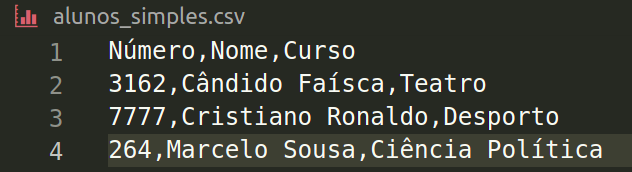
\includegraphics[width=\textwidth]{pl01.png}
\caption{Ficheiro Simples de CSV.} \label{fig1}
\end{figure}

O programa lê a primeira linha do texto corresponde ao cabeçalho.
De seguida descobre o nome dos paramêtros, sendo que os guarda em um \textit{\textbf{array de strings}}.

\vspace{5mm}
A partir do número de elementos do array constroi um espressão de captura:


\verb|(.*?),(.*?),(.*)|

\vspace{5mm}
Depois é construida a expressão de substituição dependendo do nome e do índice dos paramêtros:

\verb|{"Número": "\1","Nome": "\2","Curso": "\3"}|

\vspace{5mm}
Desta forma temos a expressão de captura e a expressão de substituição basta apenas aplicar à string no formato CSV para a converter em JSON.
\begin{equation}
jsonString = re.sub("pattern","substituion\_pattern","string")
\end{equation}


Sendo o output o seguinte:


\verb|[{"Número": "3162","Nome": "Cândido Faísca","Curso": "Teatro"} ,|
\verb|{"Número": "7777","Nome": "Cristiano Ronaldo","Curso": "Desporto"} ,|
\verb|{"Número": "264","Nome": "Marcelo Sousa","Curso": "Ciência Política"} ]|

\vspace{5mm}
Com esta abordagem criamos um simples e eficaz conversor de CSV para JSON.

\newpage
\subsection{Conversor CSV com parâmetros de tamanho variavel}


Foi nos apresentado o seguinte formato :

\begin{figure}[h]
\centering
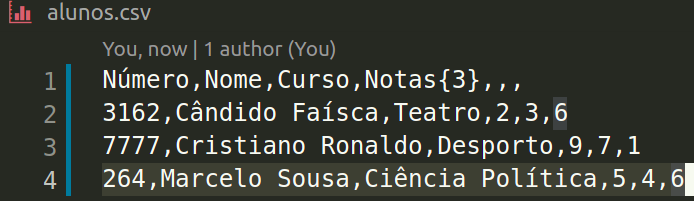
\includegraphics[width=\textwidth]{pl02.png}
\caption{Ficheiro de CSV com parâmetros variaveis.} \label{fig1}
\end{figure}


Não muito diferente da aplicação anterior foi só necessário capturar parãmetros que podem ter um tamanho variavel e ajustar a expressão de captura

\begin{verbatim}
(.*?),(.*?),(.*?),(.*?),(.*?),(.*)    
\end{verbatim}


Já para construir a expressão de substituição é necessário guardar todos os parametros numa estrutura de dados propria.


Para construir a expressão de substituição para tamanho variavel é necessário buscar o índice de começo e de fim à estrutura de dados. 

\begin{verbatim}
{"Número": "\1","Nome": "\2","Curso": "\3","Notas": [\4,\5,\6]}
\end{verbatim}

\subsection{Conversor CSV com parâmetros de tamanho variavel entre 2 inteiros}

Para o seguinte cabeçalho:


\verb|Número,Nome,Curso,Notas{1,3},,,|

A estratégia adotada foi igual à apresentada anteriormente

\newpage

\subsection{Conversor CSV com funções parametrizadas}

\begin{figure}[h]
\centering
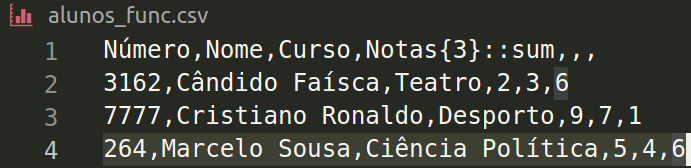
\includegraphics[width=\textwidth]{pl03.png}
\caption{Ficheiro CSV com funções associadas aos parâmetros.} \label{fig1}
\end{figure}

Para poder lidar com este parâmetro extra foi necessário guardar na nossa estrutura de dados um \textit{\textbf{ENUM}} chamado \textit{behaviour}.

\paragraph{Este behaviour pode ser atualmente de 3 tipos: \textbf{NO\_BEHAVIOUR, SUM ou MEDIA}.}

\begin{equation}
\end{equation}

Depois da operação de substituição ter sido realizada vamos iterar sobre os elementos da estrutura de dados para aplicar a função guardada em behaviour.

Tendo descoberto o novo valor realizamos uma nova substituição sobre a string em substituimos os dados anteriores pelos output da função através da seguinta função



\verb|jsonEntry = re.sub(|

\verb|fr'"{specialHeader.name}": \[.*?\]',|

\verb|fr'"{specialHeader.name}": {newnumber}',|

\verb|jsonEntry)|

\newpage

\section{Testes}

A aplicação tem uma variavel \textbf{ENABLE\_DEBUG} que por default é iniciada a \textbf{False} para não enviar para o default \textit{stdout} as strings de captura que gera.

\vspace{5mm}
Para correr o programa no terminal: 
\begin{verbatim}
    python3 csv_2_json.py ficheiro.csv
\end{verbatim}
    
\begin{figure}
    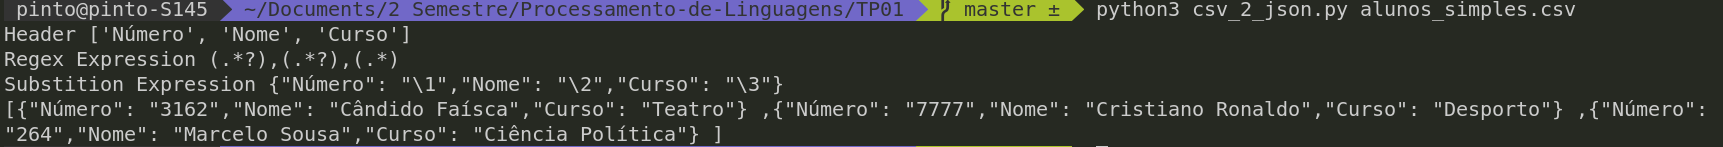
\includegraphics[width=150mm,height=25mm]{pl04.png}
    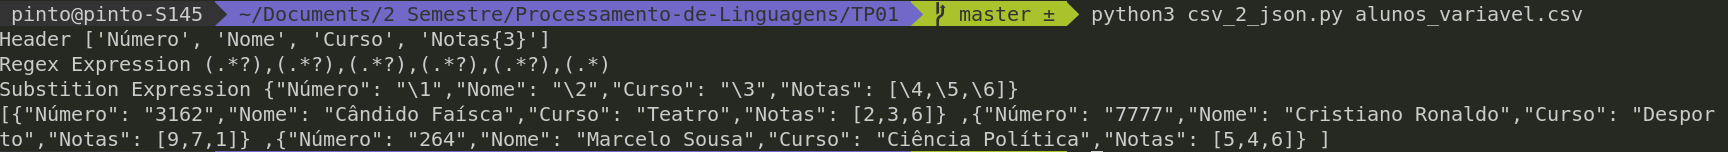
\includegraphics[width=150mm,height=25mm]{pl05.png}
    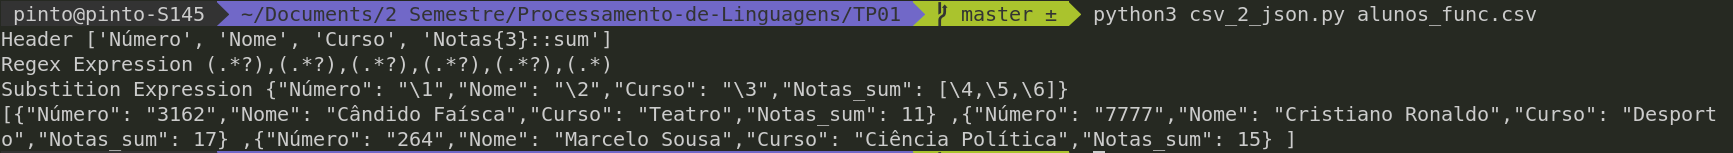
\includegraphics[width=150mm,height=25mm]{pl06.png}
\end{figure}
O programa até pode executar sem levar parametros adicionais dessa forma vai ler todas linhas do \textbf{stdin}, podemos assim aproveitar do use de \textit{pipes}.
\begin{figure}
    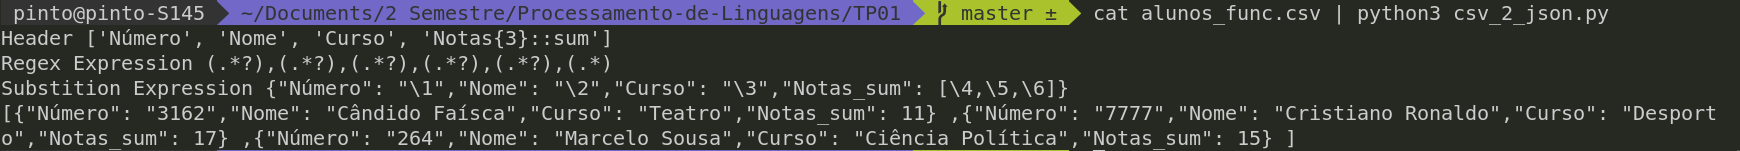
\includegraphics[width=150mm,height=25mm]{pl07.png}
\end{figure}

\newpage

\section{Conclusão}
A primeira abordagem para este problema foi de realizar uma operação de substituição sobre os dados usando a função
\begin{verbatim}
re.sub("pattern","substituion_pattern","string")
\end{verbatim}
Concluimos que esta seria a melhor abordagem devido a ser a única ferramenta que tinhamos conhecimento. Numa posterior fase de desenvolvimento foi nos apresentado nas aulas a utilização de automatos finitos e o modulo \textit{ply}.


Uma abordagem com essas ferramentas seria muito mais fácil de implementar e mais escalável. Ainda assim como já estava o trabalho quase terminado achamos melhor que iriamos continuar usando a função \textit{sub}.

\vspace{5mm}
Este trabalho foi bastante útil para \textit{meter-mos a mão na massa} e ficar confortáveis a usar expressões regulares.

\end{document}
